\begin{frame}
\frametitle{Enumeration of degrees of freedom}

\begin{itemize}
\item Numbering of DoFs necessary to build linear equation
\item Parallelization and p-adaptive methods require different algorithms
  \begin{itemize}
  \item See parallel \parencite{bangerth2012} and hp \cite{bangerth2009} papers for details
  \end{itemize}
\end{itemize}

\vspace{-.7em}
\begin{block}{\vspace{-.7em}}
\centering
Combination of both algorithms \textbf{not trivial}
\end{block}

\vfill{}

\begin{itemize}
\item Why not number DoFs locally and handle relations with constraints?
  \begin{itemize}
  \item Number of DoFs would vary with number of processors
  \item Larger matrices \& vectors, thus higher memory demand
  \end{itemize}
\end{itemize}

\vfill{}

\begin{itemize}
  \item Need for algorithm independent of number of processors
  \begin{itemize}
    \item Results independent of number of processors
    \begin{itemize}
      \item Proof that solvers work
    \end{itemize}
    \item Simplifies debugging
  \end{itemize}
\end{itemize}
\end{frame}





\begin{frame}
\frametitle{Enumeration algorithm}

\begin{itemize}
\item Developed 6-phase algorithm
  \begin{itemize}
  \item Requires two ghost exchanges
  \end{itemize}
\end{itemize}

\vfill{}

\begin{enumerate}
  \item Local enumeration of DoFs
  \item Invalidate DoFs on ghost interfaces to processors with lower rank
  \item Unification of DoFs on local domain \textbf{and} ghost interfaces
  \begin{itemize}
    \item Ownership of DoFs clarified
  \end{itemize}
  \item Global re-enumeration of DoFs
  \begin{itemize}
    \item Local DoF indices set
  \end{itemize}
  \item Exchange of locally owned DoFs
  \item Merge DoFs on ghost interfaces
  \begin{itemize}
    \item Global DoF indices set
  \end{itemize}
\end{enumerate}
\end{frame}




\let\oldthesubfigure\thesubfigure
\renewcommand{\thesubfigure}{Phase \arabic{subfigure}}

\def\Length{1}
\def\Radius{0.03}

\begin{frame}
\frametitle{Example of application of enumeration algorithm}
\begin{overprint}

\onslide<1>
\begin{figure}
  \begin{subfigure}{0.5\textwidth}
    \resizebox{\textwidth}{!}{
      \begin{tikzpicture}[scale=3.3]
  \fill[fzjlightblue] (0, 0) rectangle (2*\Length, \Length);
  \fill[fzjorange] (0, \Length) rectangle (2*\Length, 2*\Length);
  \node at (\Length, 0.7*\Length) {\Huge \textcolor{fzjblue}{\textbf{CPU 0}}};
  \node at (\Length, 1.7*\Length) {\Huge \textcolor[rgb]{0.44,0.26,0.08}{\textbf{CPU 1}}};

  \node at (0.5*\Length, 0.3*\Length) {\Huge \(Q_2\)}; 
  \node at (1.5*\Length, 0.3*\Length) {\Huge \(Q_4\)};
  \node at (0.5*\Length, 1.3*\Length) {\Huge \(Q_4\)}; 
  \node at (1.5*\Length, 1.3*\Length) {\Huge \(Q_2\)};

  \LagrangeCell{0}{0}{\Length}{\Radius}{1}
    {{"","","",""}};
  \LagrangeCell{\Length}{0}{\Length}{\Radius}{1}
    {{"","","",""}};
  \LagrangeCell{0}{\Length}{\Length}{\Radius}{1}
    {{"","","",""}};
  \LagrangeCell{\Length}{\Length}{\Length}{\Radius}{1}
    {{"","","",""}};
\end{tikzpicture}
    }
    \caption{Local enumeration}
  \end{subfigure}
  \caption{Example of application of our enumeration algorithm for degrees of freedom}
\end{figure}

\onslide<2>
\begin{figure}
  \begin{subfigure}{\textwidth}
    \resizebox{\textwidth}{!}{
      \begin{tikzpicture}[scale=3.3]
  \fill[fzjyellow] (0, 0) rectangle (2*\Length, \Length);

  \LagrangeCell{0}{0}{\Length}{\Radius}{2}
    {{0,1,2,3,4,5,6,7,8}};
  \LagrangeCell{\Length}{0}{\Length}{\Radius}{4}
    {{9,10,11,12,13,14,15,16,17,18,19,20,21,22,23,24,25,26,27,28,29,30,31,32,33}};
  \LagrangeCell{0}{\Length}{\Length}{\Radius}{4}
    {{"i","","i","i","i","i","i","i","i","i","i","i","i","i","i","i","i","i","i","i","i","i","i","i","i"}};
  \LagrangeCell{\Length}{\Length}{\Length}{\Radius}{2}
    {{"","i","i","i","i","i","i","i","i","i","i","i","i","i","i","i"}};
\end{tikzpicture}
      \hfill{}
      
\begin{tikzpicture}[scale=3.3]
  \fill[color=green] (0, \Length) rectangle (2*\Length, 2*\Length);
  
  \LagrangeCell{0}{0}{\Length}{\Radius}{2}
    {{"i","i","i","","i","i","i","i","i"}};
  \LagrangeCell{\Length}{0}{\Length}{\Radius}{4}
    {{"i","i","","i","i","i","i","i","i","i","i","i","i","i","i","i","i","i","i","i","i","i","i","i","i"}};
  \LagrangeCell{0}{\Length}{\Length}{\Radius}{4}
    {{0,1,2,3,4,5,6,7,8,9,10,11,12,13,14,15,16,17,18,19,20,21,22,23,24}};
  \LagrangeCell{\Length}{\Length}{\Length}{\Radius}{2}
    {{25,26,27,28,29,30,31,32,33}};
\end{tikzpicture}

    }
    \caption{Local enumeration}
  \end{subfigure}
  \caption{Example of application of our enumeration algorithm for degrees of freedom}
\end{figure}

\onslide<3>
\begin{figure}
  \ContinuedFloat
  \begin{subfigure}{\textwidth}
    \resizebox{\textwidth}{!}{
      \begin{tikzpicture}[scale=3.3]
  \LagrangeCell{0}{0}{\Length}{\Radius}{2}
    {{0,1,2,3,4,5,6,7,8}};
  \LagrangeCell{\Length}{0}{\Length}{\Radius}{4}
    {{9,10,11,12,13,14,15,16,17,18,19,20,21,22,23,24,25,26,27,28,29,30,31,32,33}};
  \LagrangeCell{0}{\Length}{\Length}{\Radius}{4}
    {{"i","i","i","i","i","i","i","i","i","i","i","i","i","i","i","i","i","i","i","i","i","i","i","i","i"}};
  \LagrangeCell{\Length}{\Length}{\Length}{\Radius}{2}
    {{"i","i","i","i","i","i","i","i","i","i","i","i","i","i","i","i"}};
\end{tikzpicture}
      \hfill{}
      \begin{tikzpicture}[scale=3.3]
  \fill[color=Set1-F!80] (\Length - 0.15, \Length) rectangle (\Length + 0.15, \Length + 0.15);
  
  \LagrangeCell{0}{0}{\Length}{\Radius}{2}
    {{"i","i","i","i","i","i","i","i","i"}};
  \LagrangeCell{\Length}{0}{\Length}{\Radius}{4}
    {{"i","i","i","i","i","i","i","i","i","i","i","i","i","i","i","i","i","i","i","i","i","i","i","i","i"}};
  \LagrangeCell{0}{\Length}{\Length}{\Radius}{4}
    {{0,"i",2,3,4,5,6,7,8,9,10,11,12,13,14,15,16,17,18,19,20,21,22,23,24}};
  \LagrangeCell{\Length}{\Length}{\Length}{\Radius}{2}
    {{"i",26,27,28,29,30,31,32,33}};
\end{tikzpicture}

    }
    \caption{Invalidation}
  \end{subfigure}
  \caption{Example of application of our enumeration algorithm for degrees of freedom}
\end{figure}

\onslide<4>
\begin{figure}
  \ContinuedFloat
  \begin{subfigure}{\textwidth}
    \resizebox{\textwidth}{!}{
      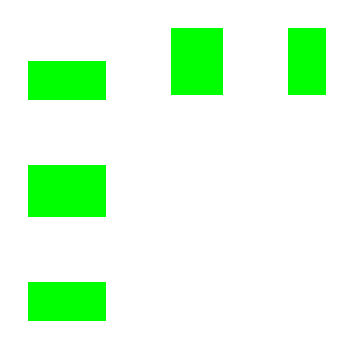
\begin{tikzpicture}[scale=3.3]
  \fill[color=green] (\Length - 0.15, 0) rectangle (\Length + 0.15, 0.15);
  \fill[color=green] (\Length - 0.15, 0.5*\Length - 0.1) rectangle (\Length + 0.15, 0.5*\Length + 0.1);
  \fill[color=green] (\Length - 0.15, \Length - 0.15) rectangle (\Length + 0.15, \Length);
  
  \fill[color=green] (1.5*\Length - 0.1, \Length - 0.13) rectangle (1.5*\Length + 0.1, \Length + 0.13);
  \fill[color=green] (2*\Length - 0.15, \Length - 0.13) rectangle (2*\Length, \Length + 0.13);
  
  \LagrangeCell{0}{0}{\Length}{\Radius}{2}
    {{0,1,2,3,4,5,6,7,8}};
  \LagrangeCell{\Length}{0}{\Length}{\Radius}{4}
    {{1,10,3,"i",13,5,15,16,17,18,19,20,21,22,"i",24,25,26,27,28,29,30,31,32,33}};
  \LagrangeCell{0}{\Length}{\Length}{\Radius}{4}
    {{"i","","i","i","i","i","i","i","i","i","i","i","i","i","i","i","i","i","i","i","i","i","i","i","i"}};
  \LagrangeCell{\Length}{\Length}{\Length}{\Radius}{2}
    {{"","i","i","i","i","i","i","i","i","i","i","i","i","i","i","i"}};
\end{tikzpicture}
      \hfill{}
      \begin{tikzpicture}[scale=3.3]
  \fill[color=Set1-F!80] (\Length - 0.15, 1.5*\Length - 0.1) rectangle (\Length + 0.15, 1.5*\Length + 0.1);
  \fill[color=Set1-F!80] (\Length - 0.15, 2*\Length - 0.15) rectangle (\Length + 0.15, 2*\Length);
  
  \fill[color=Set1-F!80] (0, \Length - 0.13) rectangle (0.15, \Length + 0.13);
  \fill[color=Set1-F!80] (0.5*\Length - 0.1, \Length - 0.13) rectangle (0.5*\Length + 0.1, \Length + 0.13);
  
  \LagrangeCell{0}{0}{\Length}{\Radius}{2}
    {{"i","i","i","i","i","i","i","i","i"}};
  \LagrangeCell{\Length}{0}{\Length}{\Radius}{4}
    {{"i","i","i","i","i","i","i","i","i","i","i","i","i","i","i","i","i","i","i","i","i","i","i","i","i"}};
  \LagrangeCell{0}{\Length}{\Length}{\Radius}{4}
    {{"i","i",2,27,4,5,6,7,29,9,10,"i",12,13,14,15,16,17,18,19,20,21,22,23,24}};
  \LagrangeCell{\Length}{\Length}{\Length}{\Radius}{2}
    {{"i",26,27,28,29,30,31,32,33}};
\end{tikzpicture}
    }
    \caption{Unification}
  \end{subfigure}
  \caption{Example of application of our enumeration algorithm for degrees of freedom}
\end{figure}

\onslide<5>
\begin{figure}
  \ContinuedFloat
  \begin{subfigure}{\textwidth}
    \resizebox{\textwidth}{!}{
      
\begin{tikzpicture}[scale=3.3]
  \fill[color=green] (0, 0) rectangle (2*\Length, \Length);
  
  \fill[white] (1.5*\Length - 0.1, \Length - 0.13) rectangle (1.5*\Length + 0.1, \Length + 0.13);
  \fill[white] (2*\Length - 0.15, \Length - 0.13) rectangle (2*\Length, \Length + 0.13);
  
  \LagrangeCell{0}{0}{\Length}{\Radius}{2}
    {{0,1,2,3,4,5,6,7,8}};
  \LagrangeCell{\Length}{0}{\Length}{\Radius}{4}
    {{1,9,3,"i",10,5,11,12,13,14,15,16,17,18,"i",19,20,21,22,23,24,25,26,27,28}};
  \LagrangeCell{0}{\Length}{\Length}{\Radius}{4}
    {{"i","i","i","i","i","i","i","i","i","i","i","i","i","i","i","i","i","i","i","i","i","i","i","i","i"}};
  \LagrangeCell{\Length}{\Length}{\Length}{\Radius}{2}
    {{"i","i","i","i","i","i","i","i","i","i","i","i","i","i","i","i"}};
\end{tikzpicture}
      \hfill{}
      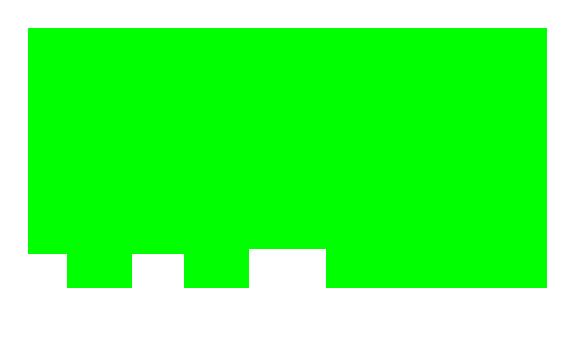
\begin{tikzpicture}[scale=3.3]
  \fill[color=green] (0, \Length) rectangle (2*\Length, 2*\Length);
  
  \fill[white] (\Length - 0.15, \Length) rectangle (\Length + 0.15, \Length + 0.15);
  \fill[white] (0, \Length - 0.13) rectangle (0.15, \Length + 0.13);
  \fill[white] (0.5*\Length - 0.1, \Length - 0.13) rectangle (0.5*\Length + 0.1, \Length + 0.13);
  
  \LagrangeCell{0}{0}{\Length}{\Radius}{2}
    {{"i","i","i","i","i","i","i","i","i"}};
  \LagrangeCell{\Length}{0}{\Length}{\Radius}{4}
    {{"i","i","i","i","i","i","i","i","i","i","i","i","i","i","i","i","i","i","i","i","i","i","i","i","i"}};
  \LagrangeCell{0}{\Length}{\Length}{\Radius}{4}
    {{"i","i",29,50,30,31,32,33,52,34,35,"i",36,37,38,39,40,41,42,43,44,45,46,47,48}};
  \LagrangeCell{\Length}{\Length}{\Length}{\Radius}{2}
    {{"i",49,50,51,52,53,54,55,56}};
\end{tikzpicture}
    }
    \caption{Re-enumeration}
  \end{subfigure}
  \caption{Example of application of our enumeration algorithm for degrees of freedom}
\end{figure}

\onslide<6>
\begin{figure}
  \ContinuedFloat
  \begin{subfigure}{\textwidth}
    \resizebox{\textwidth}{!}{
      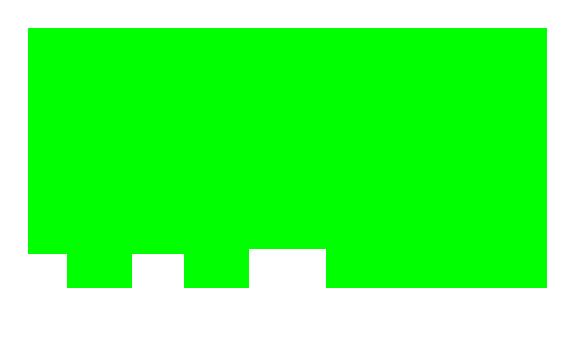
\begin{tikzpicture}[scale=3.3]
  \fill[color=green] (0,\Length) rectangle (2*\Length, 2*\Length);
  
  \fill[white] (\Length - 0.15, \Length) rectangle (\Length + 0.15, \Length + 0.15);
  \fill[white] (0, \Length - 0.13) rectangle (0.15, \Length + 0.13);
  \fill[white] (0.5*\Length - 0.1, \Length - 0.13) rectangle (0.5*\Length + 0.1, \Length + 0.13);
  
  \LagrangeCell{0}{0}{\Length}{\Radius}{2}
    {{0,1,2,3,4,5,6,7,8}};
  \LagrangeCell{\Length}{0}{\Length}{\Radius}{4}
    {{1,9,3,"i",10,5,11,12,13,14,15,16,17,18,"i",19,20,21,22,23,24,25,26,27,28}};
  \LagrangeCell{0}{\Length}{\Length}{\Radius}{4}
    {{"i","i",29,30,31,32,33,34,35,36,37,"i",38,39,40,41,42,43,44,45,46,47,48,49,50}};
  \LagrangeCell{\Length}{\Length}{\Length}{\Radius}{2}
    {{"i",51,30,52,35,53,54,55,56}};
\end{tikzpicture}
      \hfill{}
      \begin{tikzpicture}[scale=3.3]
  \fill[fzjyellow] (0,0) rectangle (2*\Length, \Length);
  
  \fill[fzjyellow] (\Length - 0.15, \Length) rectangle (\Length + 0.15, \Length + 0.15);
  \fill[white] (1.5*\Length - 0.1, \Length - 0.13) rectangle (1.5*\Length + 0.1, \Length + 0.13);
  \fill[white] (2*\Length - 0.15, \Length - 0.13) rectangle (2*\Length, \Length + 0.13);
  
  \LagrangeCell{0}{0}{\Length}{\Radius}{2}
    {{0,1,2,"",4,5,6,7,8}};
  \LagrangeCell{\Length}{0}{\Length}{\Radius}{4}
    {{1,9,"","i",10,5,11,12,13,14,15,16,17,18,"i",19,20,21,22,23,24,25,26,27,28}};
  \LagrangeCell{0}{\Length}{\Length}{\Radius}{4}
    {{"i",3,29,30,31,32,33,34,35,36,37,"i",38,39,40,41,42,43,44,45,46,47,48,49,50}};
  \LagrangeCell{\Length}{\Length}{\Length}{\Radius}{2}
    {{3,51,30,52,35,53,54,55,56}};
\end{tikzpicture}
    }
    \caption{Ghost exchange}
  \end{subfigure}
  \caption{Example of application of our enumeration algorithm for degrees of freedom}
\end{figure}

\onslide<7>
\begin{figure}
  \ContinuedFloat
  \begin{subfigure}{\textwidth}
    \resizebox{\textwidth}{!}{
      \begin{tikzpicture}[scale=3.3]
  \fill[fzjyellow] (0, \Length - 0.13) rectangle (0.15, \Length + 0.13);
  \fill[fzjyellow] (0.5*\Length - 0.1, \Length - 0.13) rectangle (0.5*\Length + 0.1, \Length + 0.13);
  \fill[fzjyellow] (1.5*\Length - 0.1, \Length - 0.13) rectangle (1.5*\Length + 0.1, \Length + 0.13);
  \fill[fzjyellow] (2*\Length - 0.15, \Length - 0.13) rectangle (2*\Length, \Length + 0.13);
  
  \LagrangeCell{0}{0}{\Length}{\Radius}{2}
    {{0,1,2,3,4,5,6,7,8}};
  \LagrangeCell{\Length}{0}{\Length}{\Radius}{4}
    {{1,9,3,51,10,5,11,12,13,14,15,16,17,18,54,19,20,21,22,23,24,25,26,27,28}};
  \LagrangeCell{0}{\Length}{\Length}{\Radius}{4}
    {{2,"",29,30,31,32,33,34,35,36,37,7,38,39,40,41,42,43,44,45,46,47,48,49,50}};
  \LagrangeCell{\Length}{\Length}{\Length}{\Radius}{2}
    {{"",51,30,52,35,53,54,55,56}};
\end{tikzpicture}
      \hfill{}
      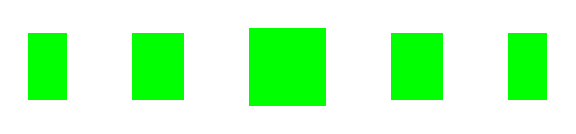
\begin{tikzpicture}[scale=3.3]
  \fill[color=green] (0, \Length - 0.13) rectangle (0.15, \Length + 0.13);
  \fill[color=green] (0.5*\Length - 0.1, \Length - 0.13) rectangle (0.5*\Length + 0.1, \Length + 0.13);
  \fill[color=green] (1.5*\Length - 0.1, \Length - 0.13) rectangle (1.5*\Length + 0.1, \Length + 0.13);
  \fill[color=green] (2*\Length - 0.15, \Length - 0.13) rectangle (2*\Length, \Length + 0.13);
  \fill[color=green] (\Length - 0.15, \Length - 0.15) rectangle (\Length + 0.15, \Length + 0.15);
  
  \LagrangeCell{0}{0}{\Length}{\Radius}{2}
    {{0,1,2,3,4,5,6,7,8}};
  \LagrangeCell{\Length}{0}{\Length}{\Radius}{4}
    {{1,9,3,49,10,5,11,12,13,14,15,16,17,18,54,19,20,21,22,23,24,25,26,27,28}};
  \LagrangeCell{0}{\Length}{\Length}{\Radius}{4}
    {{2,3,29,50,30,31,32,33,52,34,35,7,36,37,38,39,40,41,42,43,44,45,46,47,48}};
  \LagrangeCell{\Length}{\Length}{\Length}{\Radius}{2}
    {{3,49,50,51,52,53,54,55,56}};
\end{tikzpicture}

    }
    \caption{Merge}
  \end{subfigure}
  \caption{Example of application of our enumeration algorithm for degrees of freedom}
\end{figure}

\end{overprint}
\end{frame}

\renewcommand{\thesubfigure}{\oldthesubfigure}